\problem{}
\subproblem{}
قانون قوی اعداد بزرگ میگوید:\\
\[ \lim_{n \to \infty} P(\frac{X1+X2+X3+...+Xn}{n} = \mu) = 1\]
یا به بیان دیگر 
\[ \bar{X}_n \to \mu \quad a.s. \quad as \quad n\to\infty \]
\\
و یکی از مثال های جالب آن این است که در یک بازی که احتمال برد قمار باز $p$ است و احتمال برد کازینو \(1-p\) که $p<\frac{1}{2}$
پس از بازی های زیاد هرچند شاید دفعه اول قمار باز برنده باشد ولی در نهایت کازینو برنده است زیرا تعداد برد های کازینو نسبت به تعداد کل بازی ها به سمت \(1-p\) می رود که
بیشتر از $\frac{1}{2}$ است.\\

\subproblem{}
تفاوت صورت قوی و ضعیف قانون اعداد بزرگ این است که در صورت قوی آن مجموعه پشامد هایی
که در قانون صدق نمیکنند نسبت به مجموعه کل پشامد ها اندازه صفر است و این پیشامد ها ثابت و مشخص هستند
در صورتی که در صورت ضیف آن مجموعه این پیشامد ها ثابت و مشخص نیستند و این قانون میگوید صرفا با زیاد کردن تعداد
نمونه ها نسبت این پیشامد ها به مجموعه کل پیشامد ها کم و کم تر میشود اما درباره اینکه این پیشامد ها 
ثابت هستند تضمینی نمیدهد.\\\\
برهان:\\
می خواهیم نشان دهیم :\\ 
\[ \forall \epsilon >0 \quad \quad \lim_{{n \to \infty}} P(\lvert \bar{X} - \mu \rvert > \epsilon) = 0 \]
با توجه به نامساوی مارکوف داریم\\
\[P(X>a)\leq \frac{E[X]}{a} \] 
پس داریم
\[P((\bar{X} - \mu)^2>a^2)\leq\frac{E[( \bar{X} - \mu)^2]}{a^2} \] 
که این یعنی
\[P((\bar{X} - \mu)^2>a^2)\leq \frac{var(\bar{X})}{a^2} \] 
و با توجه به $i.i.d$ بودن $Xi$ ها 
\[var(\bar{X}) = \frac{\sigma^2}{n}\]
\[ P(\lvert \bar{X} - \mu \rvert > \epsilon ) \leq \frac{\sigma^2}{n\epsilon} \quad for \quad fixed \quad \epsilon \quad and \quad  \sigma<\infty\] 
پس:
\[0 \leq \lim_{{n \to \infty}} P(\lvert \bar{X} - \mu \rvert > \epsilon) \leq \lim_{{n \to \infty}} \frac{\sigma^2}{n\epsilon} = 0 \]
که ثابت میشود:
\[ \forall \epsilon >0 \quad \quad \lim_{{n \to \infty}} P(\lvert \bar{X} - \mu \rvert > \epsilon) = 0 \]

\subproblem{}
کد پایتون:\\
\begin{figure}[H]
	\centering
	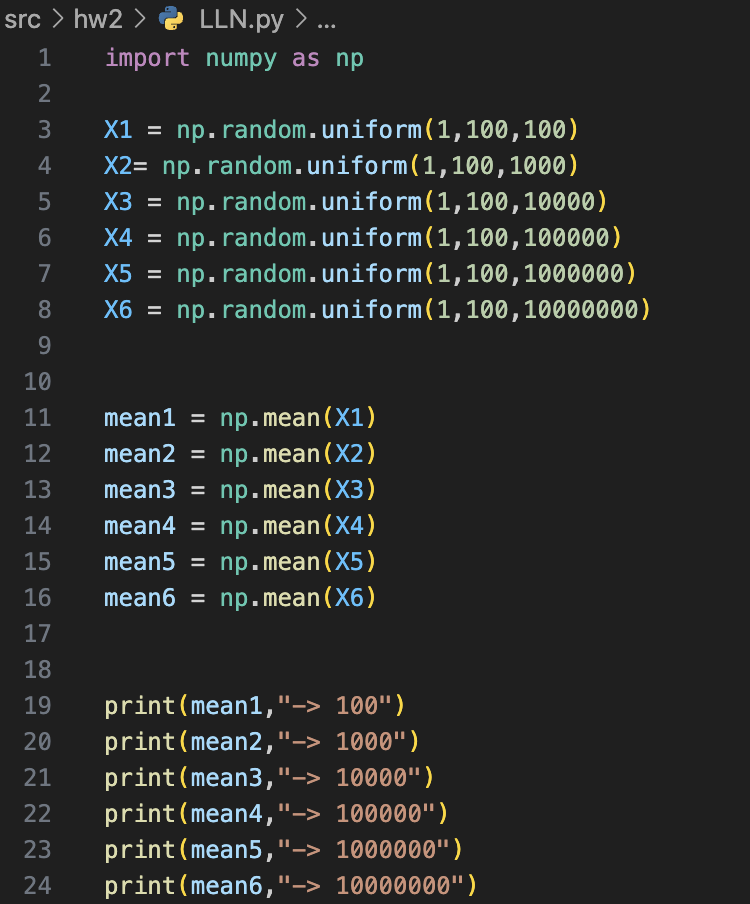
\includegraphics[width=0.5\textwidth]{/Users/kajal/Documents/statistics/resources/hw2/Figure_3.png}
\end{figure}

خروجی کد:
\begin{figure}[H]
	\centering
	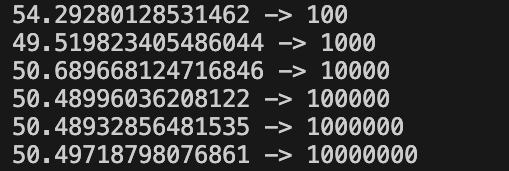
\includegraphics[width=0.5\textwidth]{/Users/kajal/Documents/statistics/resources/hw2/Figure_4.png}
\end{figure}
